\documentclass{article}

%%% Importiamo i pacchetti
\usepackage{natbib}
\usepackage{graphicx}% pacchetto per immagini centrate
\usepackage{wrapfig} % pacchetto per immagini laterali
\usepackage{placeins}% per usare floatbarrier
\usepackage{lipsum}

%%Inizializziamo il progetto
\begin{document}

%%Creiamo la sezione 
\section{Immagini}
Per usare le immagini bisogna importare 2 librerie. Per farlo si utilizza il tag \textbf{usepackage} subito dopo il tag \textbf{documentclass}. \\ 
L'immagine va caricata nel progetto 


%% Aggiungiamo una prima immagine centrale con testo sopra e sotto l'immagine
\begin{figure}[h!]
    \centering
    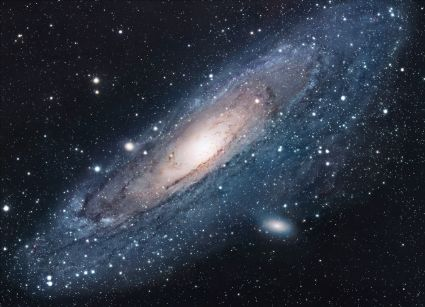
\includegraphics[scale=1.7]{img_src/universe.jpg}
    \caption{The Universe }
    \label{fig:my_label}
\end{figure}
\FloatBarrier


%centering          ->  tag che centra l'immagine
%includegraphics    ->  [grandezza immagine]{path dell'immagine}
%caption            ->  testo descrittivo immagine
%label              ->  referenza immagine 

Possiamo creare una referenza all'immagine tramite il tag \textbf{ref}:\\
Figura \ref{fig:my_label}


\begin{wrapfigure}{l}{0.4\textwidth}
    \centering
    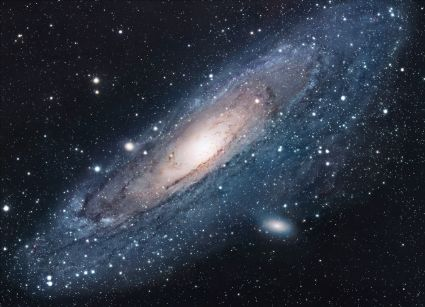
\includegraphics[width=0.4\textwidth]{img_src/universe.jpg}
    \caption{The Universe }
    \label{fig:unilaterale}
\end{wrapfigure}
\FloatBarrier

\lipsum[2-4]

%% Indice delle figure presenti nel progetto
\listoffigures


\end{document}